\section{Publish/Subscribe-Systeme}
\label{chap:grundlagen:pubsub}
\missing{schöner: Zur Verteilung von Events (Event-Dissemination) gibt es vielfältige Systeme, wie MessagePassing .. many faces!}

Publish/Subscribe-Systeme sind Forschungszweck vieler wissenschaftlicher Arbeiten (z.B. \cite{Banerjee2001Comparative, Liu2003Survey, Muhl2002LargeScale, FiegeSecurity, Castro2002Scribe}) und daher gut erforscht und beschrieben. Diese Systeme eigenen sich auf Grund ihres Aufbaus sehr gut zur Eventverteilung in dezentralen Systemen, da sie gegenüber anderen Nachrichtensystemen (wie z.B. \emph{message passing} oder \emph{rpc}) in drei orthogonalen Dimensionen\index{Publish/Subscribe!orthogonale Dimensionen} skalieren \cite{PatrickTh2003Many}.

\begin{figure}[htbp]
\centering
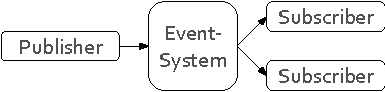
\includegraphics{grafics/pubsub_black_box.pdf}
\caption{Schema eines Publish/Subscribe-Systemes.}
\label{fig:pubsub_black_box}
\end{figure}

\paragraph{räumliche Trennung}
Wie in \Fref{fig:pubsub_black_box} zu sehen ist, trennt das Event-System Publisher und Subscriber räumlich voneinander. Diese Trennung bezieht sich nicht alleine auf verschiedene Schichten einer Applikation, sondern kann auch über Applikationsgrenzen oder gar Rechnergrenzen gehen. \missing{Kommunikationsparadigmen, send and forget}\\
Weiterhin skaliert ein solches System besser, da der Publisher nur mit dem Event-System kommuniziert und dieses darauf ausgelegt ist, viele Subscribern zu bedienen.



Diese Trennung kann so weit gehen, dass verschiedene Publish/Subscribe-Systeme miteinander kommunizieren können. \cite{PiEyKoSh2007-PubSubAPI} gibt einen Vorschlag für eine generische API\index{Publish/Subscribe!generische API} für Publish/Subscribe-Systeme und unterteilt die Kompabilität verschiedener Systeme in drei Level. Das höchste Level beschreibt einen Datenaustausch der an XML-RPC angelegt ist.

\paragraph{zeitliche Trennung}
Publisher und Subscriber sind in ihren Aktionen mit dem Event-System zeitlich getrennt. Ein Publisher muss kein Wissen über Subscriber haben und umgekehrt. Dies bedeutet dass sich ein Subscriber am System anmelden kann, obwohl kein Publisher vorhanden ist. Für Publisher gilt dies analog. Bei \emph{message-passing} ist dies nicht möglich, da die Gegenseite bekannt sein muss.

\missing{CITE für message-passing}

\paragraph{asynchrone Verarbeitung}
Das Senden einer Nachricht ist für den Publisher nicht blockierend. Die Auslieferung der Nachricht erfolgt für die Subscriber ebenfalls nicht blockierend, da ihnen die Nachricht per Callback zugestellt wird und damit die Verarbeitung vom Event-System aus getriggert wird.


\subsection{Arten von Publish/Subscribe-Systemen}
Publish/Subscribe-Systeme gibt es grundsätzlich in zwei Ausführungen:
\begin{itemize}
\item kanalbasiert (\emph{topic-based})
\item filterbasiert (\emph{content-based})
\end{itemize}

Beide Varianten haben grundsätzlich andere Arbeitsweisen, die nun näher beschrieben werden.

\subsubsection{Kanalbasiert}
\label{chap:grundlagen:pubsub:kanalbasiert}
Nachrichten in kanalbasierten\index{Publish/Subscribe!kanalbasiert} Systemem werden im Kontext von Kanälen oder Topics behandelt. Nachrichten können nur in Verbindung mit einem Topic an das System übergeben werden. Clients können sich für verschiedene Kanäle einschreiben und erhalten nur diese Nachrichten.
\missing{Das ist nicht schön beschrieben!}

Listing \vref{code:pubsub-topicbased} zeigt die mögliche API eines solchen Systemes, diese variiert aber von System zu System. Jedoch ist klar ersichtlich, dass die API stark vom Kanalnamen geprägt ist. \emph{deliver\_callback} bezeichnet hier eine Funktion, die das System bei neuen Nachrichten aufrufen soll.

\lstinputlisting[caption={Exemplarische API eines topic-based Event-Systems}, label=code:pubsub-topicbased]{listings/pubsub_topicbased.cpp}

Kanalbasierte Systeme können sehr gut optimiert werden, da die Anzahl der Kanäle und deren Art zur Erstellungszeit meist bekannt ist. Selbst wenn zur Laufzeit neue Kanäle hinzugefügt werden, geschieht dies ebenfalls strukturiert und dient der internen Optimierung des Systems. Durch die Gruppierung der Nachrichten, müssen insgesamt weniger Nachrichten verschickt werden.

Filterungen sind in diesem Systemen meist nur clientseitig effizient möglich. Clients können die empfangenen Nachrichten filtern und unpassende Nachrichten verwerfen. Wird eine Filterung durch strukturierte Kanalnamen, wie z.B. \emph{TEAMSPEAK.TEAM\_EAGLE} oder \emph{TEAMSPEAK.TEAM\_RED}, ermöglicht, kann die Anzahl der zu versendenden Nachrichten reduziert wreden. Möchte ein Client alle \emph{TEAMSPEAK}-Nachrichten empfangen, muss für jeden Kanal eine eigene Subscribtion am System erfolgen.

Um das System im Vorraus filtern zu lassen, müsste ein geeigneter Filter bei der Anmeldung übergeben werden. Damit das Event-System die Nachrichten filter kann, müssen diese in einem vom System lesbaren Format vorliegen. Dies bedeutet, dass das Event-System und die Clients stärker gekoppelt sind oder dass durch selbstbeschreibende Nachrichtenformate die Nachrichtengröße aufgebläht wird.\\
\cite{PiEyKoSh2007-PubSubAPI} zeigt mit einem System aus XML basierten Nachrichten und XPath Filter das dies möglich ist. Weiterhin verbessert dies, wie oben angesprochen, die Interopabilität verschiedener Systeme.

Können keine selbstbeschreibende Nachrichtenformate genutzt werden, so müssen dem Event-System Callbacks zur Filterung zur Verfügung stehen. Diese Callback können jedoch erst auf Clientseite ausgeführt werden, was einen Transport der Nachricht zum Client bedingt. Dies widerspricht jedoch der Idee der Nachrichtenvermeidung durch Filterung. In \Fref{chap:konzeption_pubsub} wird beschrieben, wie solch eine Filterung jedoch auch gewinnbringend eingesetzt werden kann.

Ein prominenter Vertreter dieser Art ist Scribe \cite{Castro2002Scribe}, dessen Funktionsweise in \Fref{chap:related:scribe} genau beschrieben wird.

\subsubsection{Filterbasiert}
\label{chap:grundlagen:pubsub:filterbased}
In filterbasierten\index{Publish/Subscribe!filterbasiert} Systemen, gibt es streng genommen nur einen einzigen Kanal. Bei der Anmeldung muss der Client ein Prädikat übergeben. Das Event-System liefert nur die Nachrichten aus, die darauf passen. Wie oben beschrieben, muss das Event-System zur Filterung die Nachrichten lesen können, bzw. müssen diese mit filterbaren Metadaten angereichert werden.\\
Listing \ref{code:pubsub-contentbased} zeigt in Anlehnung an \cite{PiEyKoSh2007-PubSubAPI} eine exemplarische API für solche Systeme. Statt eines Kanalnames wird bei der Subscription ein Filter übergeben. Über das zurückgegebene Handle kann sich ein Client wieder abmelden.

Filterbasierte Systeme sind nicht im gleichen Ausmaße optimierbar wie kanalbasierte Systeme, da jeder Client potentiell alle Nachrichten empfangen kann. Durch eine Anpassung der Filter sind diese Systeme jedoch flexibler in der Benutzung.

\lstinputlisting[caption={Exemplarische API eines content-based Event-Systems}, label=code:pubsub-contentbased]{listings/pubsub_contentbased.cpp}

\missing{MEHR! Attribute und Wertebereich beim Systemstart fix vs. variabel zur Laufzeit $\rightarrow$ Auswirkung auf Systemaufbau}

\subsection{Umsetzung verteilter Publish/Subscribe-Systeme}
Anhand Scribe (kanalbasiert) \cite{Castro2002Scribe} und Mercury (filterbasiert) \cite{Bharambe2004Mercury} wird die Umsetzung der in diesem Kapitel vorgestellten Arten in strukturierten Overlay-Netzwerken beschrieben. Obwohl sich \ac{m2etis} im jetzigen Entwicklungsstand auf kanalbasierte Systeme beschränkt, kann der Algorithmuns hinter Mercury interessante Einblicke und Ideen liefern.

\subsubsection*{Multicast-Tree am Beispiel von Scribe}
\label{chap:related:scribe}
Eine Umsetzung von Publish/Subscribe-Systemen in verteilen Systemen, ist der Aufbau eines Multicast-Trees\index{Multicast-Tree}, d.h. eines durch die Knoten im Netz gebildeten Baumes in dem die Nachrichten verteilt werden. Hierbei wird pro Kanal ein eigener Multicast-Tree aufgebaut. Am Algorithmus von Scribe wird diese Struktur beschrieben.

Scribe basiert auf dem strukturierten Overlay-Netzwerk Pastry \cite{Rowstron2001} und erzeugt einen vom Subscriber zum Publischer aufgebauten Baum \emph{reverse path forwarding tree} \cite{Dalal1978}.

\begin{figure}[htbp]
\centering
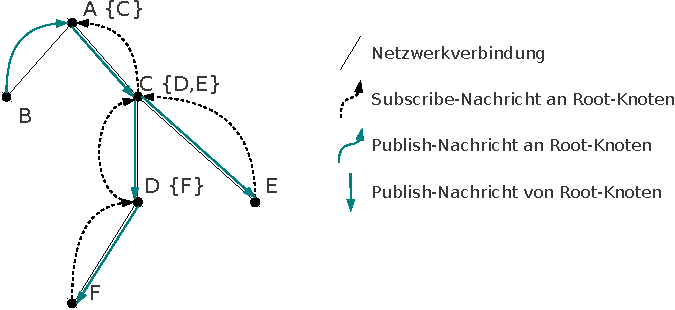
\includegraphics{grafics/multicast_tree.pdf}
\caption{Schema eines Multicast-Trees}
\label{fig:multicast_tree}
\end{figure}

\Fref{fig:multicast_tree} zeigt ein Netzwerk mit den sechs Knoten A-F. Die Verbindungen der Knoten werden durch dünne schwarze Linien dargestellt. Beispielsweise hat Knoten C Verbindungen zu A, B, D und F.\\
Der Multicast-Tree benötigt einen Knoten, der die Wurzel (im Folgenden \emph{Root-Knoten} genannt) darstellt. Aus Hashwert des Kanalnamens wird ein Schlüssel berechnet. Derjenige Knoten, der für aufgrund der Netzwerkmetrik für diesen Schlüssel zuständig ist, wird Root-Knoten des Kanals. Im abgebildeten Falle ist dies Knoten A.\\
Weiterhin hält jeder Knoten eine Liste bei ihm angemeldeter Knoten. In der Abbildung wird diese Liste durch geschweifte Klammern nach der Knotenbezeichnung dargestellt.

\paragraph*{Subscribe}
Knoten F sendet eine \emph{subscribe}-Nachricht an A. Diese Nachrichten sind in der Grafik durch gebogene schwarze Verbindungslinien mit Pfeil dargestellt. Das Netwerk würde diese Nachricht über Knoten D und C an A routen. Knoten D lässt die Nachricht terminiern und trägt F in die Liste der Subscriber ein. Knoten D sendet nun selbst eine subscribe-Nachricht an A. C, über den die Nachricht geroutet wird, terminert diese, trägt D in die Liste ein sendet selbst eine subscribe-Nachricht an A. A erhält nun diese Nachricht und trägt C in die Liste ein. Damit sind nun ingesamt drei Nachrichten verschickt worden.\\
Wenn sich Knoten E für den Kanal einschreibt, wird die subscribe-Nachricht an A über dne Knoten C geleitet. Dieser terminiert die Nachricht und fügt E der Liste hinzu. Da C selbst angemeldet ist, muss keine weitere Nachricht versendet werden.

Scribe fordert periodische Subscriptions zur Erhöhung der Fehlertoleranz.

\paragraph*{Unsubscribe}
Der Austritt aus einem Kanal erfolgt ähnlich zur Subscribtion. Die Nachrichten laufen nur bis zum nächsten Knoten und terminieren dort. Der Knoten entfernt den Sender der Nachricht aus seiner Liste und sendet selbst nur eine \emph{unsubscribe}-Nachricht, wenn die Liste leer ist und er selbst nicht angemeldet ist.

\paragraph*{Publish}
In \Fref{fig:multicast_tree} möchte Knoten B eine Nachricht im Kanal publizieren. B sendet darauf eine Nachricht an den Root-Knoten A, da dieser für diesen Kanal zuständig ist (gebogene türkise Linie). Nun sendet A diese Nachricht an alle Knoten in seiner Liste (gerader türkiser Pfeil). Dies ist in der Abbildung nur Knoten C. Dieser sendet sie weiter an D und E. E gibt diese Nachricht direkt an die Applikation weiter, während D die Nachricht an F schicken muss.


\paragraph*{Schwächen}
Hierbei ist klar ersichtlich, dass ein Overhead an Nachrichten entsteht, wenn Knoten F eine Nachricht im Kanal publizieren möchte. Diese Nachricht muss erst von Knoten F zu Knoten A wandern, nur damit A diese Nachricht wieder über die anderen Knoten zurücksendet. Optimierte Versionen dieses Algorithmus können hier ansetzen und zu publizierende Nachrichten nicht mehr an den Knoten senden, der ihnen diese Nachricht geschickt hat. So würde C die Nachricht gleich an E weiterleiten.


Obwohl dieses System die Anzahl der zu versendenden Nachrichten drastisch reduziert, ist anzumerken, dass Knotenpunkte Kanalnachrichten bearbeiten müssen, für die sie sich nicht interessieren. Beispielsweise ist Knoten A in \emph{TEAM RED}, ist aber berechneter Root-Knoten des Kanals \emph{TEAMSPEAK.TEAM\_EAGLE}.


\paragraph*{Filterung}
Eine Filterung der Nachrichten ist möglich. Im einfachsten Falle, wird der Filter bei jedem Subscriber geprüft, im komplexeren Falle werden die Filter der Subscriber mit zum Root-Knoten geschickt und die Zwischenknoten kombinieren die empfangenen Filter zu einem generellen Filter. Somit ist es möglich, dass eine Nachricht gar nicht an einen Subtree gesendet werden muss.


\paragraph*{Eignung}
Ein Multicast-Tree ist für weittragende beziehungsweise übergreifende Nachrichten wie Teamspeak oder Systemnachrichten gut gegeignet. Für lokal bezogene Nachrichten (z.B. Positionsupdate) skaliert dieses System jedoch schlecht, da jede einzelne Positionsnachricht alle angemeldeten Knoten ins Netz gesandt wird, jedoch nur für einen Bruchteil relevant ist. Eine Filterung, wie oben angesprochen, ist nicht sinnvoll, da benachbarte Knoten nicht unbedingt aus Spielesicht benachbart sind. Somit kann die Anzahl der zu versendenden Nachrichten nicht reduziert werden.\\
Da Knoten nur die Positionsupdates ihrer Nachbarn benötigen, ist es eine Möglichkeit, dass sich ein Knoten nur bei seinen Nachbarn anmeldet. Zwar müssen in einem Overlay-Netzwerk, die Nachrichten immer noch über andere Knoten verschickt werden, jedoch wird die Anzahl der Hops und Nachrichten geringer sein.



Bayeux \cite{Zhuang2001} ist ein ähnliches System, jedoch auf Basis des Overlay-Netzwerkes Tapestry. Da beide dieser Netwerke der generischen API entsprechen, stellt dies keinen Unterschied dar. Im Gegensatz zu Scribe, erzeugt Bayeux einen Baum der vom Publisher zum Subscriber aufgebaut wird. Aufgrund der unterliegenden Routingstruktur des genutzten Overlay-Netzwerkes können sich diese Pfade unterscheiden.\\
\ac{von} geht hier einen ähnlichen aber vom Aufbau des Netzwerkes anderen Ansatz. In diesem Netzwerk ist ein Nachbar in der virtuellen Welt direkt auch ein Nachbar im Netzwerk. Der Nachrichtenaustausch erfolgt nur mit den Nachbarn \cite{Hu2006VON}. \ac{vast} \cite{Backhaus2007Voronoibased} greift das Konzept von \ac{von} auf und testet eine Implementierung auf OpenSIM \cite{Baumgart2007OverSim}.



\subsubsection{Content-based am Beispiel von Mercury}
\label{chap:related:mercury}
Mercury \cite{Bharambe2004Mercury} gehört zur Klasse der filterbasierten Publish/Subscribe-Systeme\index{Publish/Subscribe!filterbasiert}.

\paragraph*{Arbeitsweise}
Im System gibt es eine Menge an Attributen, die ihrerseits einen definierten Wertebereich haben. Jedes Attribut wird durch einen eigenen \emph{Hub} gebildet. Ein Hub ist ein Verbund aus Knoten, die untereinander über Nachbarschaftsmetriken\footnote{Alte Version: forward- und backward-Pointer; Ringstruktur\\Neue Version: Tabelle mit allen Knoten im Hub} verknüpft sind. Der Wertebereich ist dabei nicht zwingend symmetrisch\footnote{Angenommen, $0<=x<360$: Knoten $A_{[0,270)}$, $B_{[270, 360)}$} auf die Knoten verteilt.

Eine Subscription $S$ ist ein Tupel aus Filterbedingungen über die Attribute (z.B. $S := (5 < x <= 20; y = 15)$) sowie Kontaktinformationen des Knotens. $S$ wird an einen beliebigen Knoten eines Hubs gesendet, der für das Attribut aus der Filterbedingung mit der größten Selektivität zuständig ist. Im Beispiel ist dies Attribut $y$. Im Hub wird $S$ nun zu dem Knoten weitergereicht, der den Wertebereich der Filterung abdeckt. Dort wird $S$ in einer Liste gespeichert.

Eine Publikation $P$ ist ebenfalls ein Tupel mit bestimmten Werten der Attribute (z.B. $P := (x = 10; y = 0)$). $P$ wird an \emph{alle} Hubs gesendet und dort zum zustädnigen Knoten weitergereicht. Dieser prüft nun die Liste der gespeicherten Subscriptions gegen die neue Publikation. Stimmen beide überein, so wird $P$ an den eingeschriebenen Knoten weitergeleitet.

\paragraph*{Offene Punkte}
\begin{itemize}
\item Änderung der Attribute zur Laufzeit?
\item Auswahl der Knoten für einen Hub?
\item Aufteilung der Wertemenge auf die Knoten?
\item (imho keine Aussage über die Knotenverbindungen)
\end{itemize}

Mirinae ist ein ebenfalls ein content-based Publish/Subscribe-System, stellt den Wertebereich eines Attributes jedoch als Hyperwürfel da, in dem Knoten mehrere Ecken/Kanten darstellen. Eine automatische Anpassung dieser Aufteilung ermöglicht ein schnelles und kurzes Routen der Nachrichten \cite{Choi2005Mirinae}.
